\documentclass[12pt, a4paper]{article}
\usepackage[francais]{babel}
\usepackage{caption}
\usepackage{graphicx}
\usepackage[T1]{fontenc}
\usepackage{listings}
\usepackage{geometry}
\usepackage[colorlinks=true,linkcolor=black,anchorcolor=black,citecolor=black,filecolor=black,menucolor=black,runcolor=black,urlcolor=black]{hyperref}

% \usepackage{mathpazo} --> Police à utiliser lors de rapports plus sérieux

\usepackage{fancyhdr}
\pagestyle{fancy}
\lhead{}
\rhead{}
\chead{}
\rfoot{\thepage}
\lfoot{Martin Baumgaertner}
\cfoot{}

\renewcommand{\headrulewidth}{0.4pt}
\renewcommand{\footrulewidth}{0.4pt}

\begin{document}
\begin{titlepage}
	\newcommand{\HRule}{\rule{\linewidth}{0.5mm}} 
	\center 
	\textsc{\LARGE iut de colmar}\\[6.5cm] 
	\textsc{\Large SAE3 - ROM}\\[0.5cm] 
	\textsc{\large Année 2022-23}\\[0.5cm]
	\HRule\\[0.75cm]
	{\huge\bfseries Déployer un service de téléphonie}\\[0.4cm]
	\HRule\\[1.5cm]
	\textsc{\large martin baumgaertner}\\[6.5cm] 

	\vfill\vfill\vfill
	{\large\today} 
	\vfill
\end{titlepage}
\newpage
\tableofcontents
\newpage
\section*{Contexte}
L'objectif de cette SAE et de créer un service de téléphonies "multi-sites". Je
m'explique. Nous allons devoir créer, un serveur Asterisk qui est un serveur de
téléphonie IP. Ce serveur est installé sur une machine virtuelle Debian11. Nous
avons aussi à disposition, 2 téléphones IP matériel qui sont des téléphones SIP. Ces
téléphones sont connectés dans le même réseau que notre serveur IPBX bien entendu. 
Puis, nous avons un troisième téléphone IP mais cette fois-ci sous forme de softphone
qui est un téléphone SIP qui est installé sur un ordinateur. Nous utiliserons 
Linphone. Ce dernier est un logiciel libre et gratuit. Il est disponible sur
Windows, Linux et Mac. Ce softphone est connecté sur le même réseau que notre serveur
IPBX.\\

Chaque membre de la SAE doit choisir un contexte de travail différent. J'ai pour
ma part choisi d'être la table 1, le médecin généraliste. De plus, nous 
avons donc ces 3 postes IP pour illustrer un vrai cabinet. C'est-à-dire que nous
avons un poste physique pour le praticien, un poste physique pour l'assistant et
le softphone pour le secretariat.\\

\section{Objectif 1}
\subsection{Configuration Serveur IPBX}
	\subsubsection{Créer une machine virtuelle Debian11}
	Pour cette SAE, j'ai décidé de choisir d'utiliser VMWare Workstation car c'était
	le logiciel que nous utilisions en cours surtout pendant les TP réseaux en première
	année. J'ai donc crée une VM Debian11. 

	\subsubsection{Installez l'IPBX asterisk via le système de paquets Debian}
	Pour pouvoir installer asterisk, il faut d'abord installer le paquet suivant :\\
	
	\texttt{sudo apt install asterisk}\\

	Une fois Asterisk installé, pour l'utiliser il faut arrêter le service pour pouvoir
	démarrer Asterisk car sinon il y a un conflit. Pour arrêter le service, il faut
	écrire la commande suivante : \texttt{service asterisk stop}. Ensuite, nous
	pouvons démarrer Asterisk avec la commande suivante : \texttt{asterisk -vvvvc}.


	\subsubsection{Pour le service IPBX, déclarez les différents postes SIP}
	Pour déclarer les différents postes SIP, j'ai donc écris les commandes suivantes
	dans les fichiers de configuration de Asterisk.\\

	Premièrement, \textbf{pjsip.conf} :
	\begin{figure}[h]
		\centering
		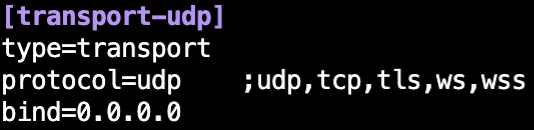
\includegraphics[width=0.6\textwidth]{img/pjsip.png}
		\caption{Configuration de pjsip.conf}
		\label{fig:pjsip}
	\end{figure}\\
	Ce sont des entrées de configuration pour la définition d'un transport 
	PJSIP dans le fichier de configuration d'Asterisk.
	\begin{itemize}
		\item \textbf{[transport-udp]} définit un nom pour le transport, "transport-udp" en l'occurrence.\\
		\item \textbf{type = transport} indique le type de l'objet de configuration. Ici, il s'agit d'un transport PJSIP.\\
		\item \textbf{protocol = udp} définit le protocole de transport utilisé, en l'occurrence l'UDP (User Datagram Protocol).\\
		\item \textbf{bind = 0.0.0.0} définit l'interface réseau sur laquelle le transport écoutera les connexions. La valeur "0.0.0.0" signifie que le transport écoutera sur toutes les interfaces disponibles.\\
	\end{itemize}

	\newpage 
	

	Puis, \textbf{pjsip wizard.conf} :
	\begin{figure}[h]
		\centering
		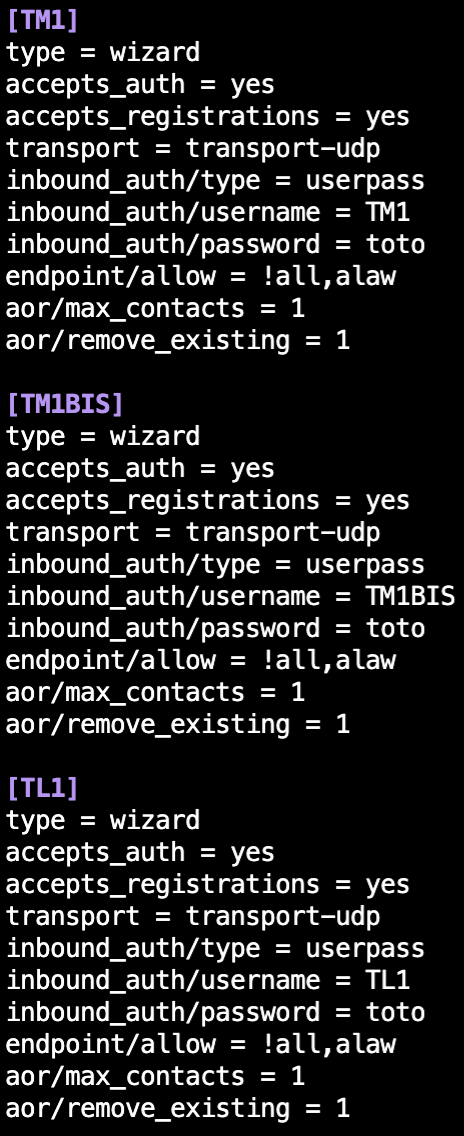
\includegraphics[width=0.4\textwidth]{img/wizard.png}
		\caption{Configuration de pjsip wizard.conf}
		\label{fig:wiz}
	\end{figure}\\

	Nous avons ici donc la configuration de tous les téléphones. A chaque fois, j'ai
	donc déclaré un téléphone avec son numéro de téléphone, son mot de passe et son
	nom d'utilisateur. Certaines lignes permettent de faire différentes choses
	essentielles au bon fonctionnement du serveur Asterisk, je vais détailler 
	toutes les explications à la page suivante. 

	\subsubsection*{Explication des lignes de configuration}
	Je vais prendre pour exemple l'utilisateur \textbf{[TL1]} car c'est après
	assez similaire pour les autres déclarations d'utilisateurs. 

	\begin{itemize}
		\item \textbf{[TL1]} : définit un nom pour l'endpoint, "TL1" en l'occurrence.\\
		\item \textbf{accepts\_auth = yes} et \textbf{accepts\_registrations = yes} autorisent l'authentification et l'enregistrement des utilisateurs pour cet endpoint.\\
		\item \textbf{transport = transport-udp} définit le transport PJSIP à utiliser pour acheminer les appels à travers le réseau pour cet endpoint.\\
		\item \textbf{inbound\_auth/type = userpass} définit le type d'authentification pour les appels entrants à cet endpoint, en l'occurrence l'authentification par nom d'utilisateur et mot de passe.\\
		\item \textbf{inbound\_auth/username = TL1} et \textbf{inbound\_auth/password = toto} définissent le nom d'utilisateur et le mot de passe pour l'authentification.\\
		\item \textbf{endpoint/allow = !all,alaw} définit les codecs audio autorisés pour les appels entrant et sortant à partir de cet endpoint. \textbf{alaw} est un codec audio couramment utilisé et \textbf{!all} signifie que tous les autres codecs ne sont pas autorisés.\\
		\item \textbf{aor/max\_contacts = 1} et \textbf{aor/remove\_existing = 1} définissent les paramètres de gestion des connexions pour cet endpoint. \textbf{Aor/max\_contacts = 1} signifie qu'un seul contact peut être enregistré pour cet endpoint à tout moment, tandis que \textbf{aor/remove\_existing = 1} signifie que les connexions existantes seront supprimées lorsqu'une nouvelle connexion est établie.\\
		\item \textbf{endpoint/call\_group = 1} et \textbf{endpoint/pickup\_group = 1} définissent les groupes d'appels et de prise en charge pour cet endpoint. Les numéros d'identification des groupes peuvent varier selon votre configuration.\\
	\end{itemize}


	Un \textbf{endpoint} est peut être un téléphone IP, un softphone, 
	une interface de téléphonie sur un ordinateur, ou tout autre appareil 
	capable de communiquer avec le système de téléphonie Asterisk.
	
	\newpage
	\subsubsection{Pour le service IPBX, créer le plan de numérotation}
	J'ai donc crée le plan de numérotation de la même manière que nous l'avons vu en cours
	et en TP comme peut en témoigner la capture d'écran suivante en rajoutant bien 
	entendu ces lignes dans le contexte \texttt{[default]} :
	\begin{figure}[h]
		\centering
		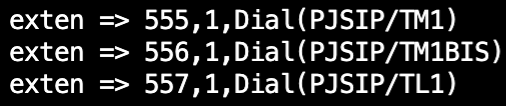
\includegraphics[width=0.7\textwidth]{img/extensions.png}
		\caption{Configuration de extensions.conf}
		\label{fig:ext}
	\end{figure}\\
	J'ai choisi de réutiliser dans un premier temps les numéros que l'on utilisait
	en cours pour me faciliter la compréhension. Ce sont des numéros, que j'ai à terme 
	modifié en 1, 2 et 3.\\

	\textbf{Exten => 555,1} définit le numéro de l'extension à 555. Lorsqu'un 
	appel est effectué à cet extension, les instructions suivantes seront 
	exécutées. \textbf{Dial(PJSIP/TM1)} est l'instruction pour composer un 
	appel. \textbf{Dial} est une commande intégrée d'Asterisk qui permet de 
	composer un appel vers une destination donnée. \textbf{PJSIP/TM1} est la 
	destination de l'appel.
	
	\textbf{PJSIP} désigne le protocole de téléphonie IP utilisé 
	(dans ce cas, PJSIP) et \textbf{TM1} est le nom de l'endpoint ou 
	de l'utilisateur auquel l'appel doit être dirigé.

\subsection{Configuration Téléphone Clients}
	\subsubsection{Téléphone logiciel Linphone}
	Tout d'abord j'ai voulu configurer linphone sur la machine windows de l'IUT
	sur laquelle j'ai fait ma VM Debian. Cependant, j'ai eu de nombreux problèmes
	Linphone ne fonctionnait pas, même après avoir essayé plusieurs versions. 
	J'ai donc essayé d'utiliser mon ordinateur personnel pour faire cette 
	manipulation. J'ai donc installé Linphone sur mon ordinateur personnel et 
	ça a fonctionné. Pour faire marcher Linphone j'ai utilisé la configuration suivante : \textit{Où 10.129.10.164 est l'IP de mon serveur Asterisk}
	\begin{figure}[h]
		\centering
		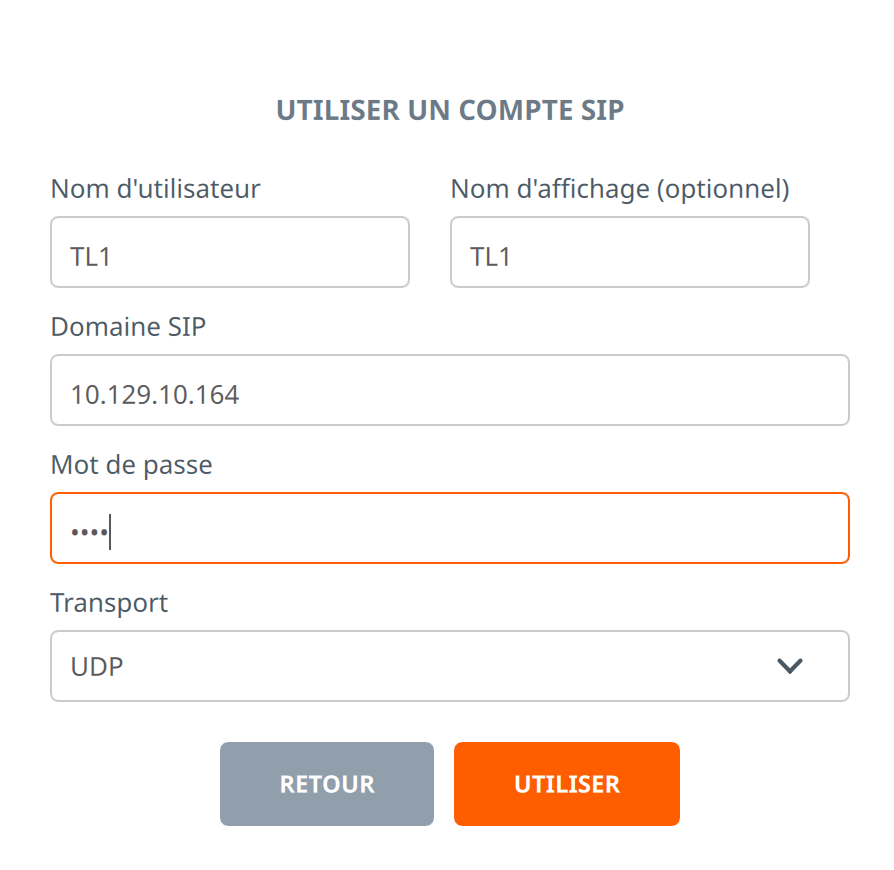
\includegraphics[width=0.5\textwidth]{img/linphone.png}
		\caption{Configuration de Linphone}
		\label{fig:lin}
	\end{figure}\\

	\subsubsection{Téléphone matériel Nortel LIP6812}
	\subsubsection*{Inscrivez le téléphone auprès du registrar de l'IPBX}
	Pour enregistrer le téléphone IP LG Nortel auprès du serveur IPBX, j'ai du
	le configurer directement depuis son interface pour rentrer tous les paramètres 
	pour qu'il puisse se connecter. \\
	Voici les différents paramètres que j'ai dû configurer pour que le téléphone remonte :
	J'ai du rentrer dans les paramètres du téléphone en appuyant sur la touche 
	\textbf{settings}, puis choisir le sous menu 2. \textbf{SIP configuration}
	\begin{figure}[h]
		\centering
		\rotatebox{-90}{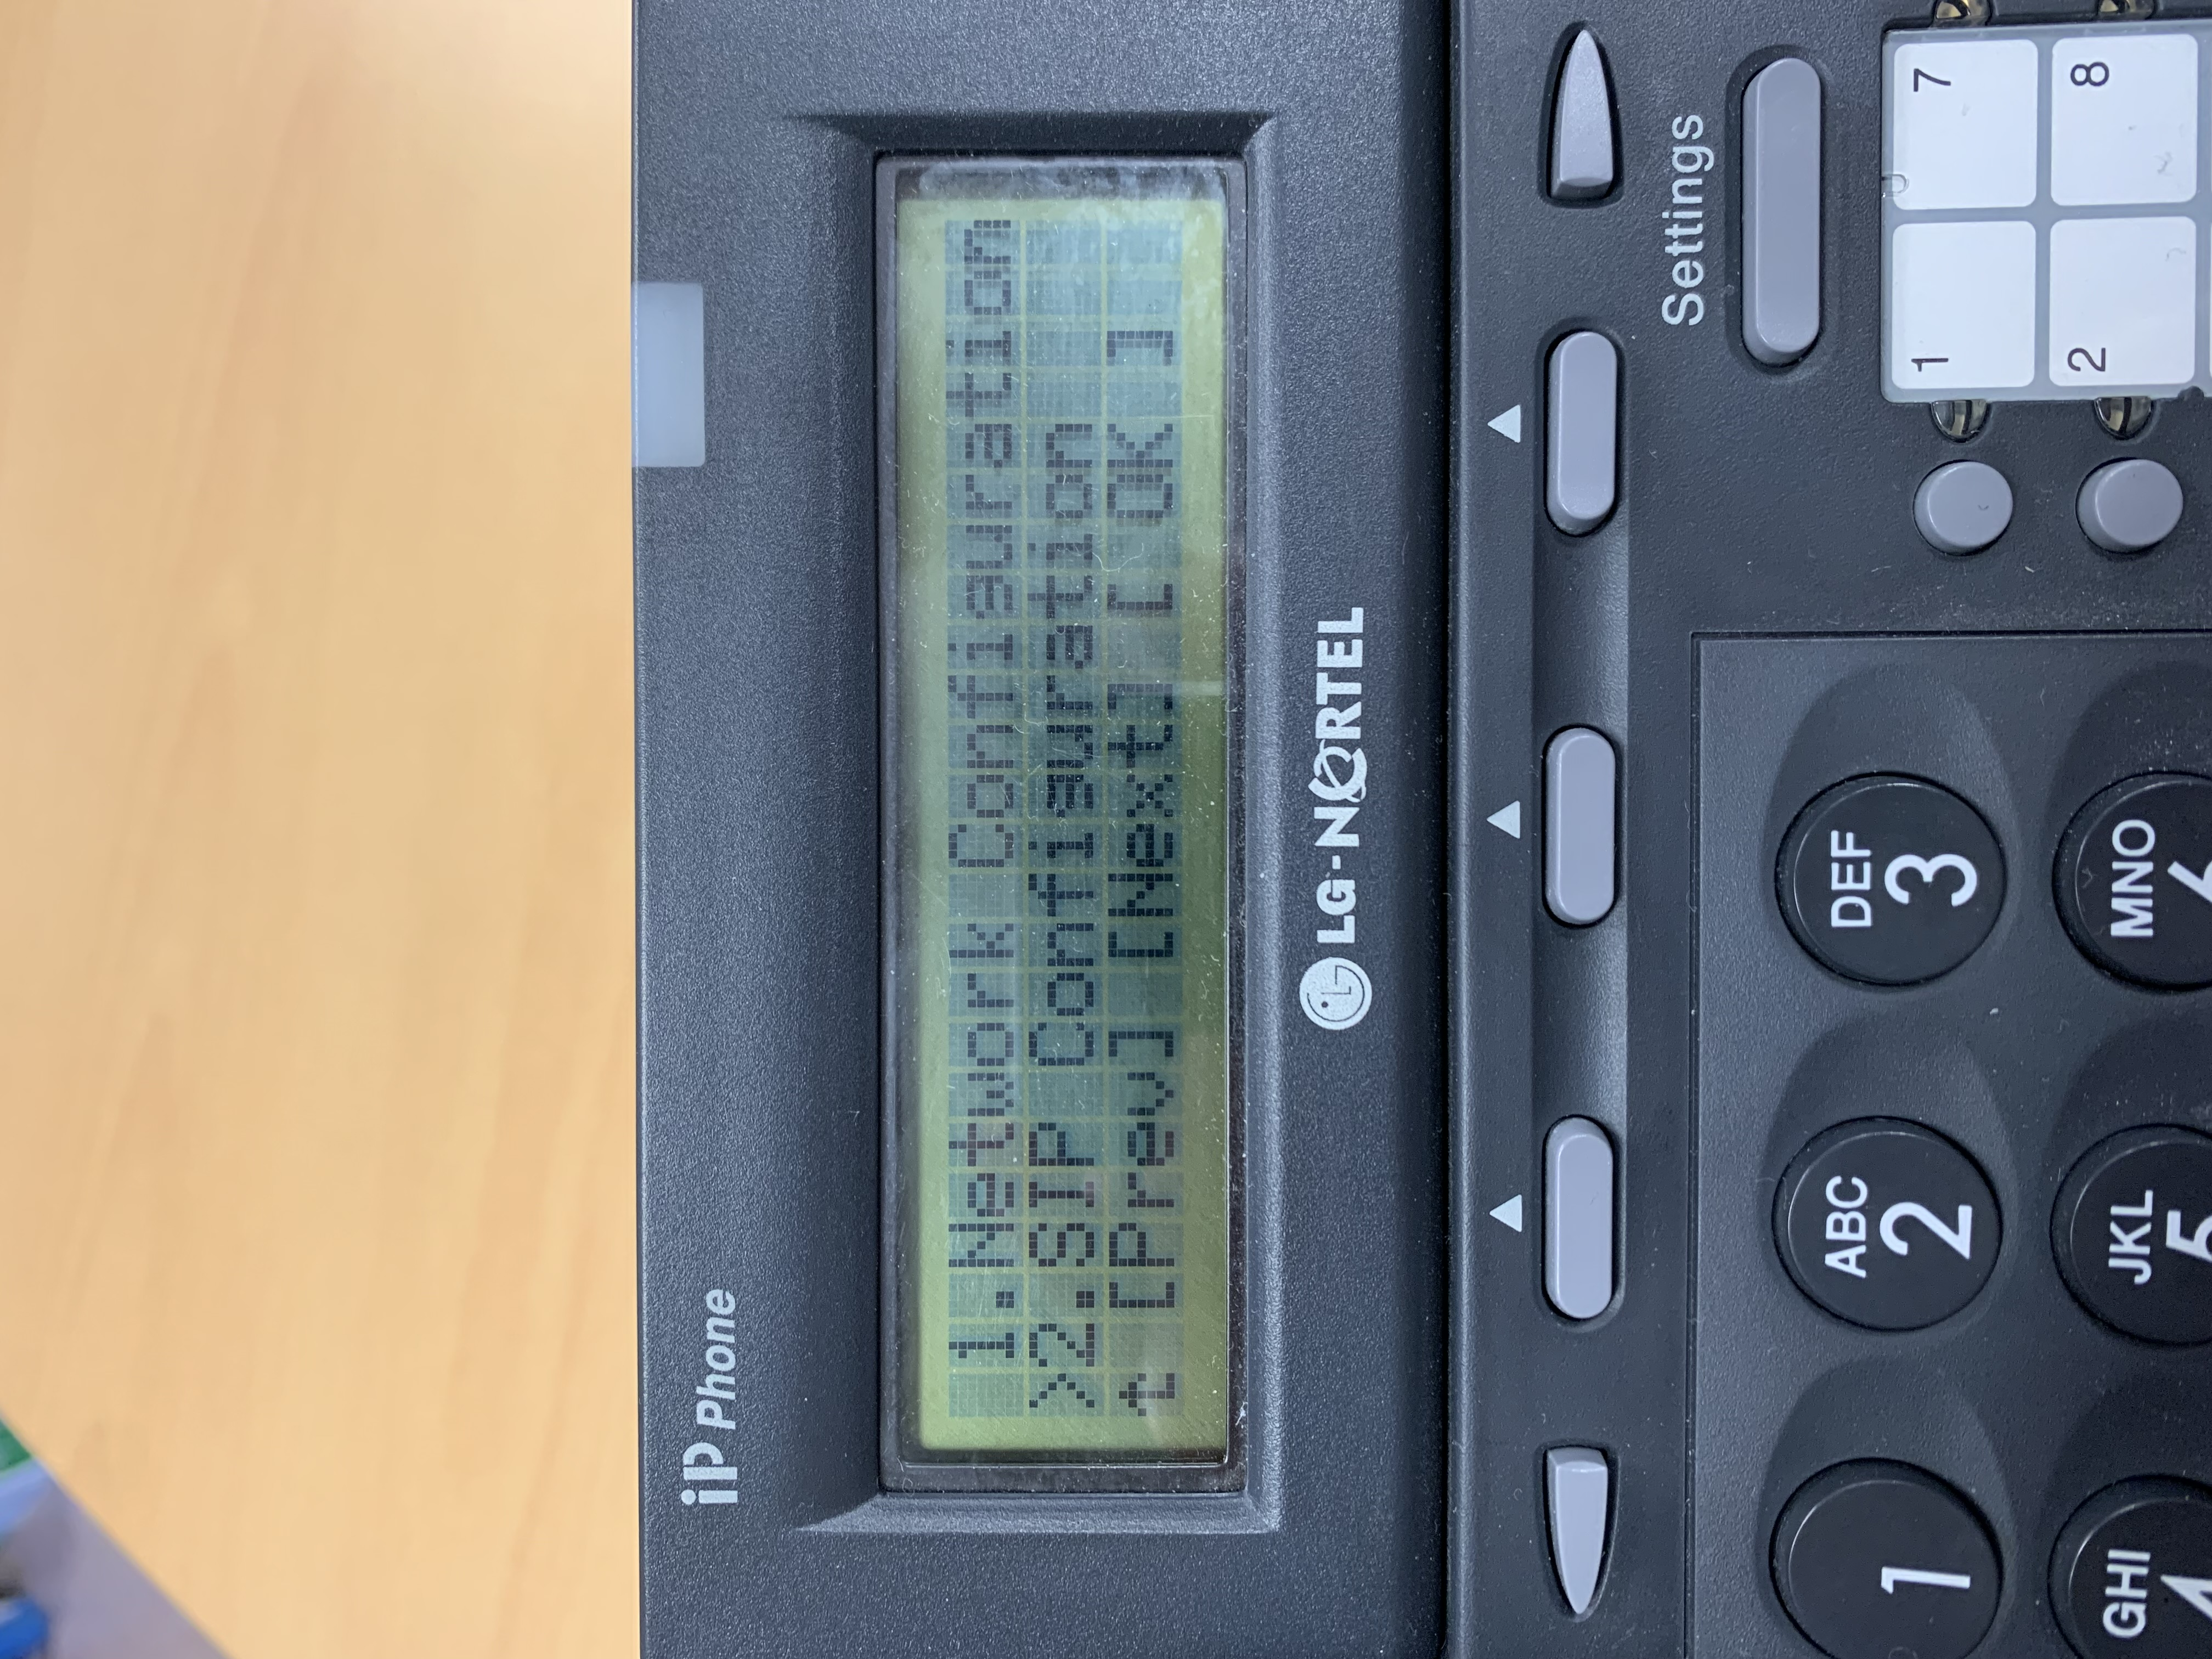
\includegraphics[width=0.4\textwidth]{img/IMG_0512.jpeg}}
		\caption{Choix menu SIP configuration}
		\label{fig:set}
	\end{figure}\\
	Ensuite, je viens sélectionner la ligne 1. \textbf{Line 1 Settings}
	\begin{figure}[h]
		\centering
		\rotatebox{-90}{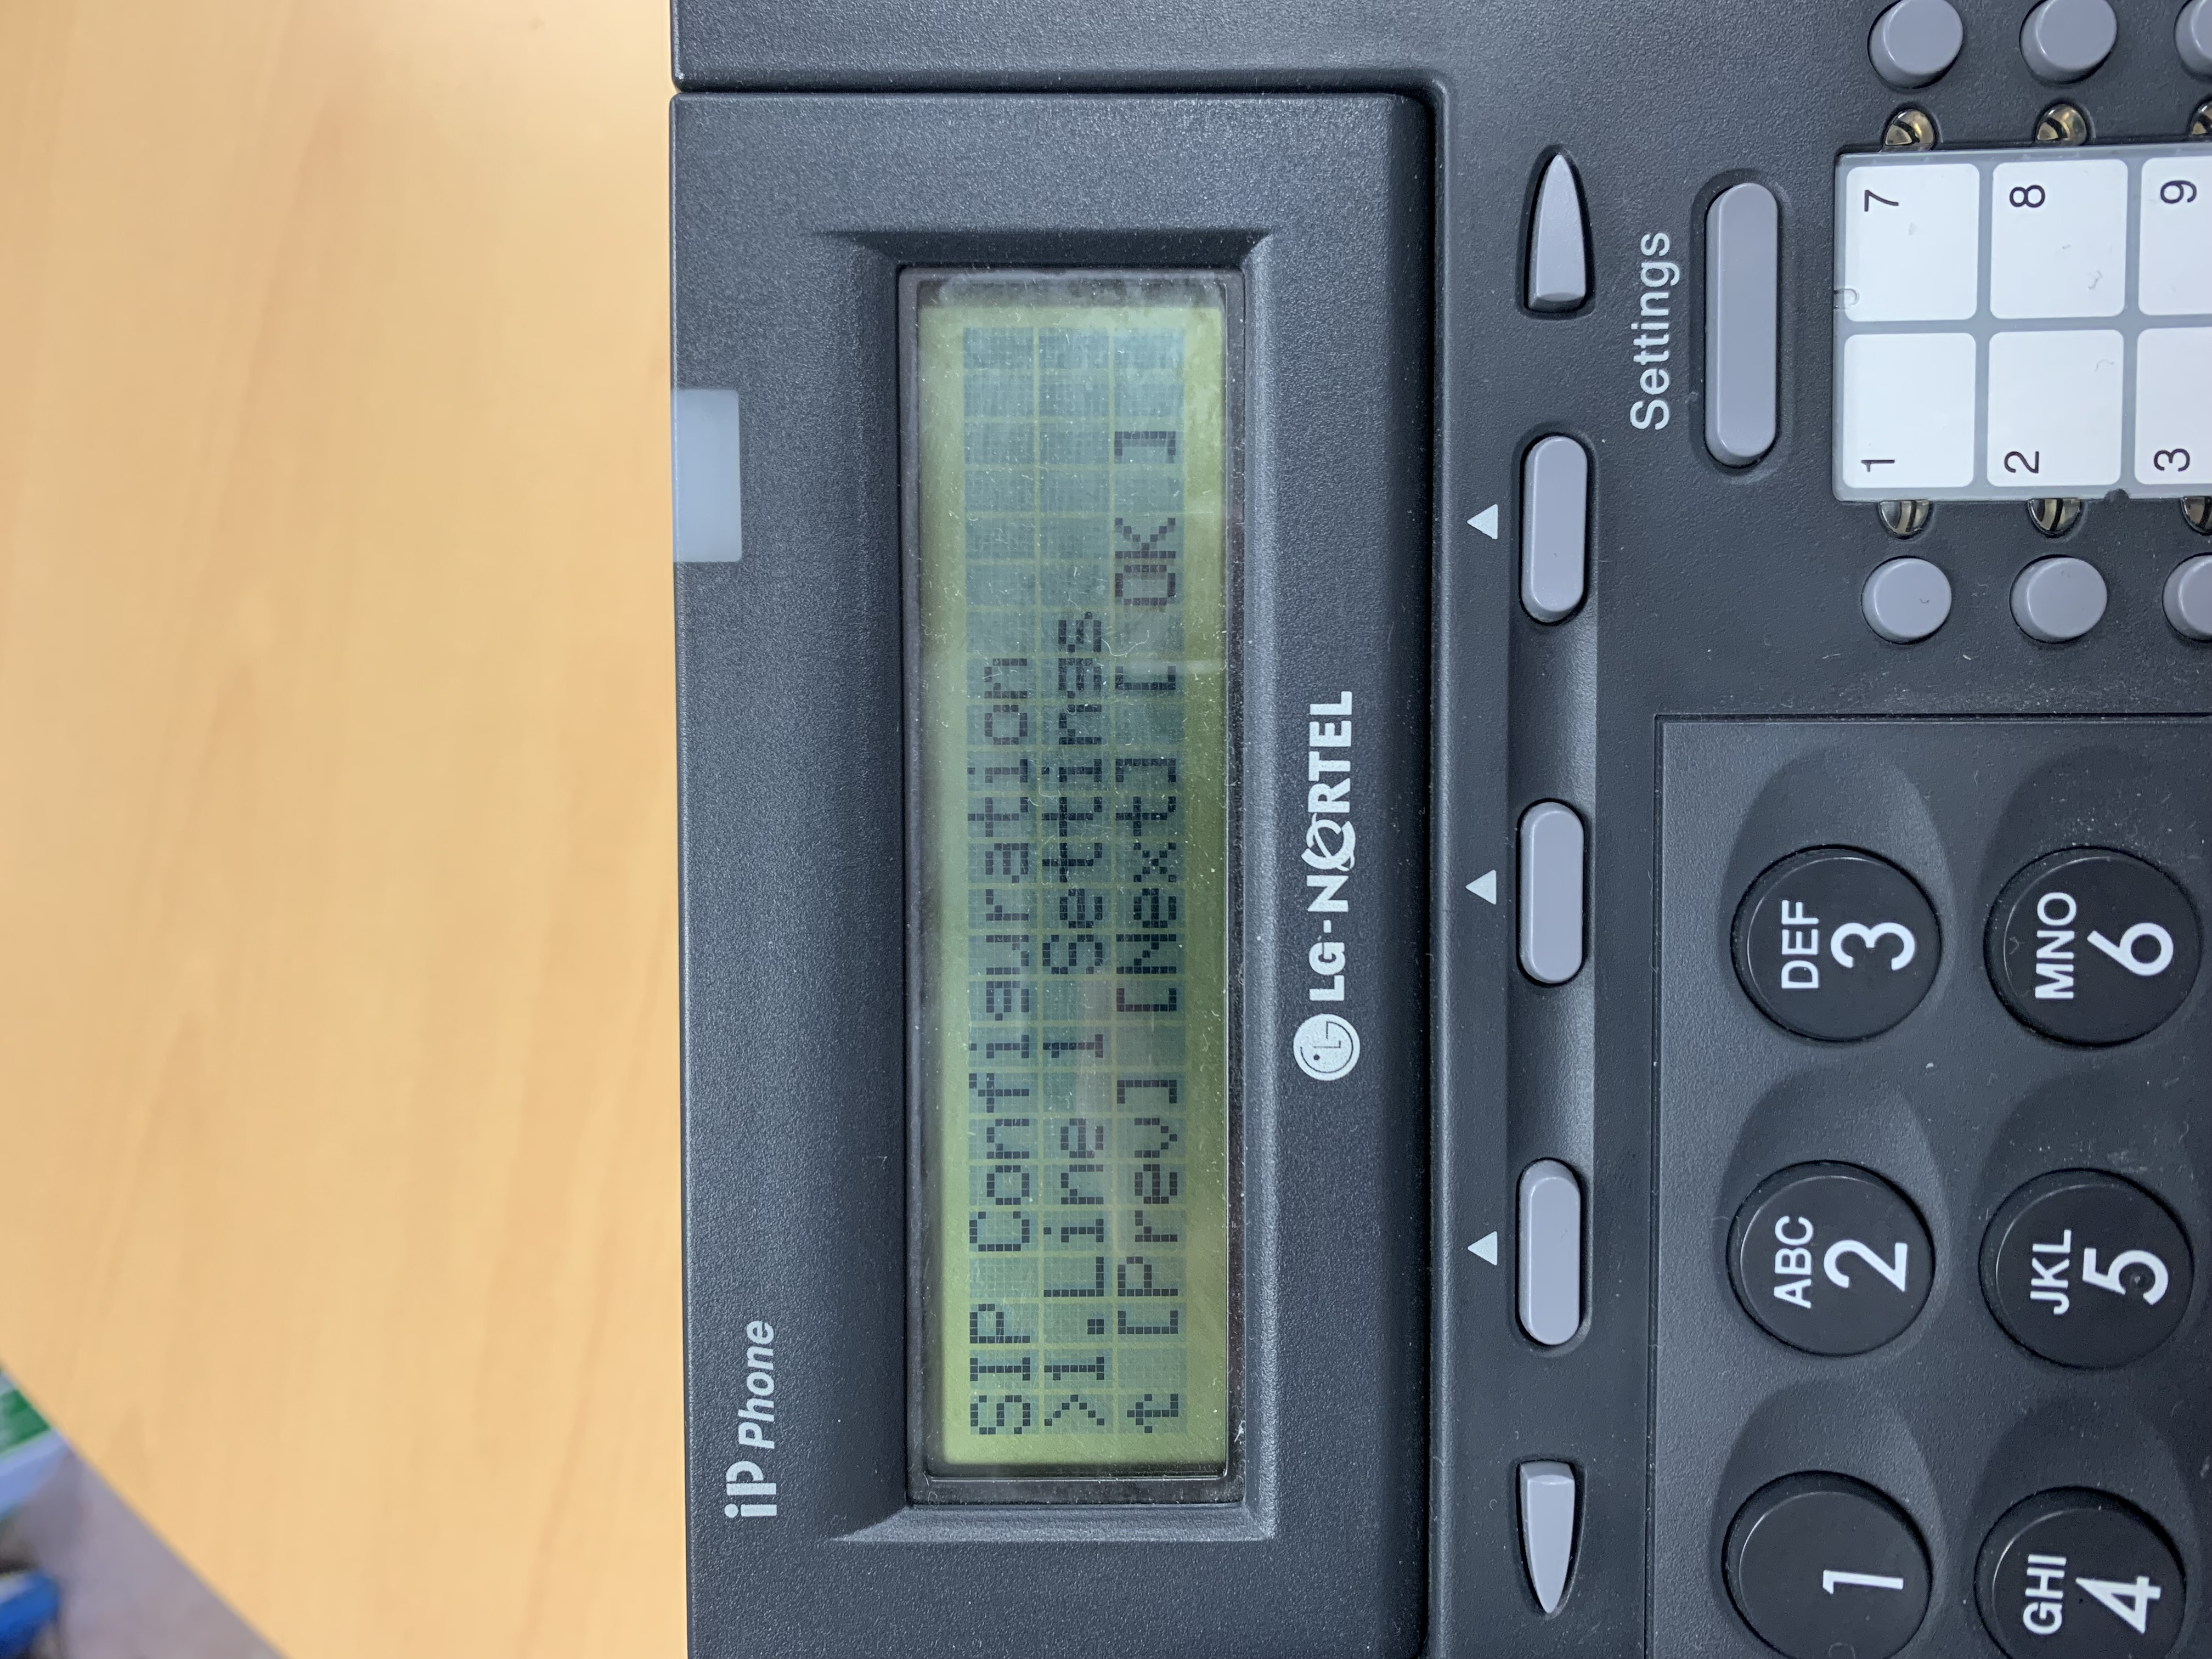
\includegraphics[width=0.4\textwidth]{img/IMG_0513.jpeg}}
		\caption{Choix menu Line 1 settings}
		\label{fig:set}
	\end{figure}\\
	Pour finir, je viens configurer l'ensemble des paramètes qui sont inscrits
	comme par exemple, l'adresse IP du serveur IPBX, le nom d'utilisateur,
	le mot de passe ainsi de suite...\\
	\begin{figure}[h]
		\centering
		\rotatebox{-90}{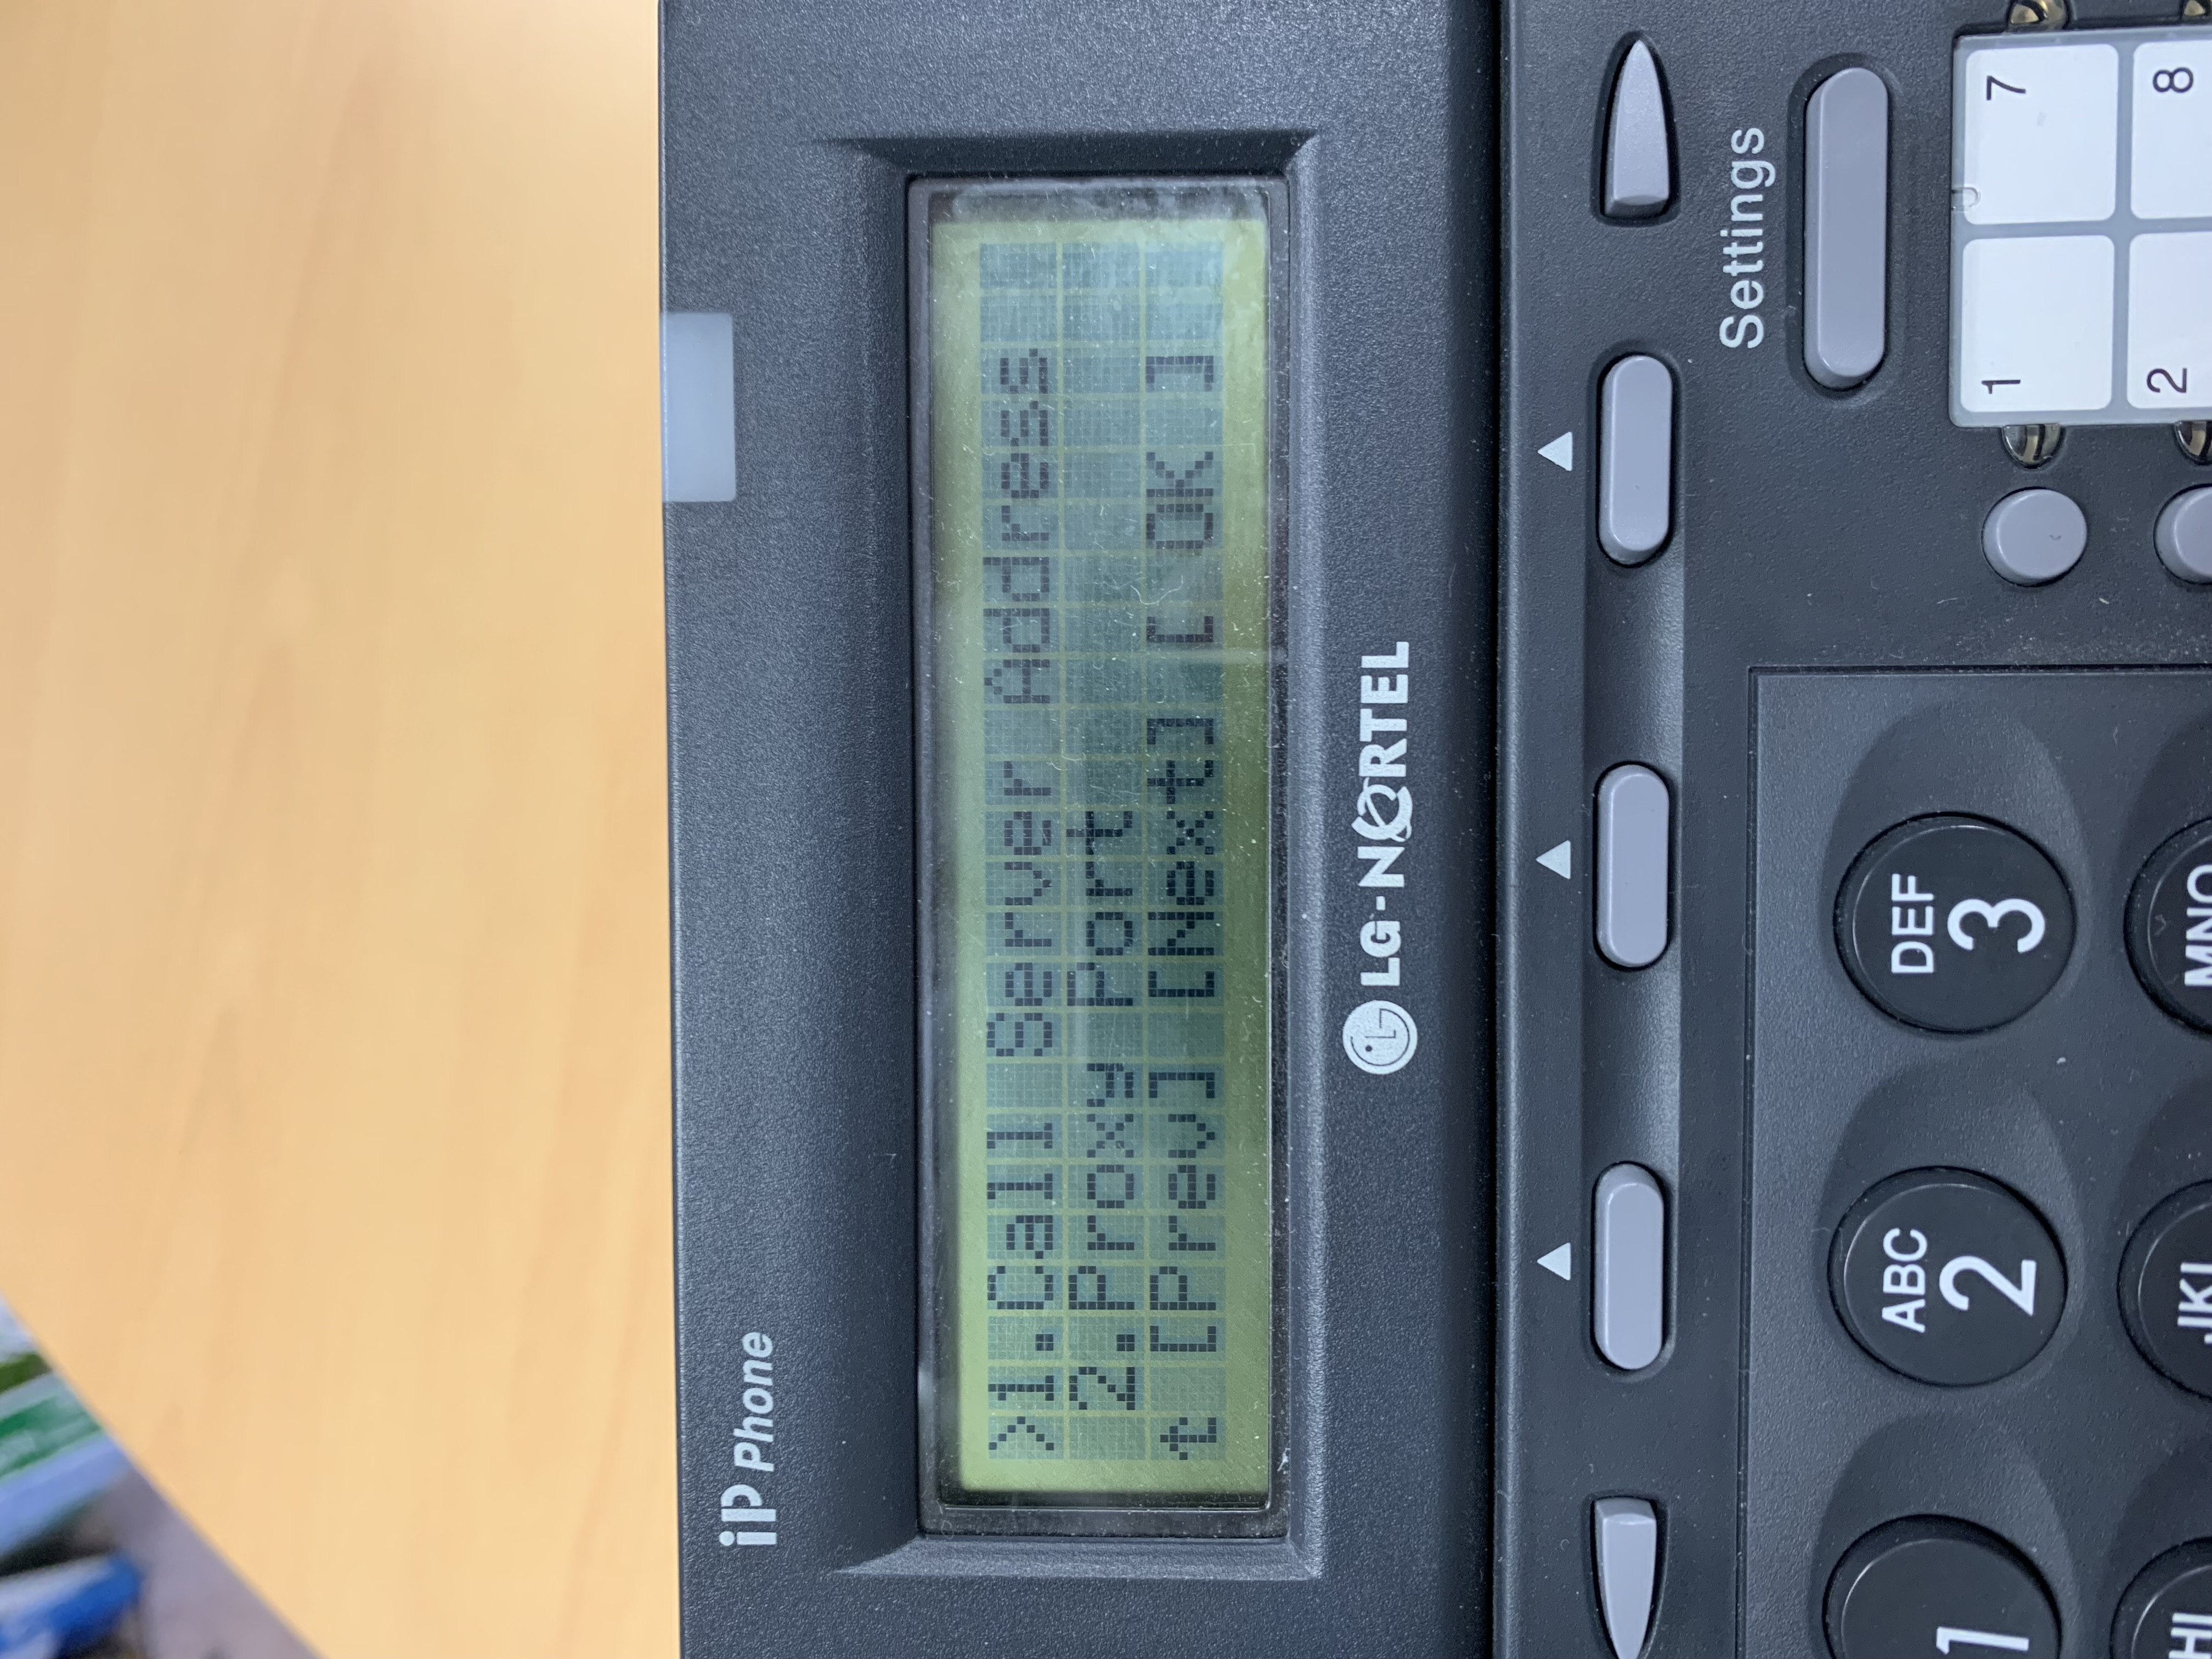
\includegraphics[width=0.4\textwidth]{img/IMG_0514.jpeg}}
		\caption{Configuration du Nortel}
		\label{fig:set}
	\end{figure}\\
	Une fois configuré correctement le téléphone remonte automatiquement auprès
	du serveur IPBX et nous pouvons l'utiliser pour appeler en interne. 


	\subsubsection{Téléphone Matériel Cisco 7941G}
	\subsubsection*{Etudiez la procédure d'installation d'un nouveau firmware}

	\subsubsection*{Installez, avec toutes les précautions nécessaires, le dernier firmware SIP}

	\subsubsection*{Inscrivez le téléphone auprès du registar de l'IPBX}
	
	\subsubsection*{Parametrez les touches d'appels rapides et collez des étiquettes}

\subsection{Validation des appels}
Nous avons donc testé les différents appels internes possibles, et tout 
est fonctionnel, j'arrive bien à joindre la secrétaire, depuis le 
softphone et inversenement. 

\newpage
\section{Objectif 2 : Configuration inter-sites}
	\subsection{Appels inter-sites}
	\subsubsection{Sur l'IPBX, inscrire le faiceau SIP}
	Pour inscrire mon faisceau SIP auprès de l'opérateur Voix, j'ai 
	configuré un nouveau contexte \textbf{[operateurvoix]} et que j'ai configuré
	comme ci-arpès : 

	\begin{figure}[h]
		\centering
		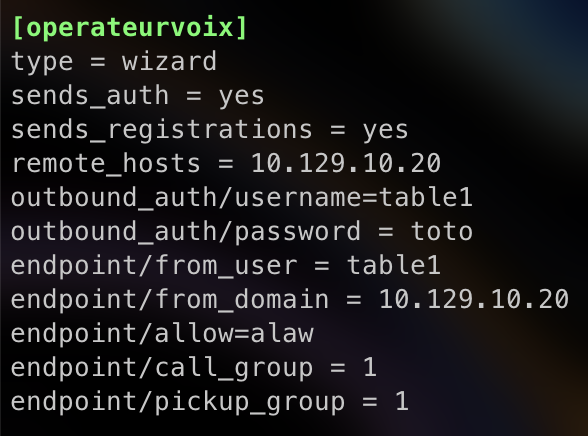
\includegraphics[width=0.4\textwidth]{img/inter.png}
		\caption{Configuration de l'opérateur Voix}
		\label{fig:opvoix}
	\end{figure}
	Je définis à chaque fois les bons paramètres que je vais expliquer ci-après :
	\begin{itemize}
		\item \texttt{remote\_hosts} : Définis l'adresse IP du serveur Opérateur Voix
		\item \texttt{outbound\_auth} : Définis le nom d'utilisateur et le mot de passe pour communiquer à travers le serveur voix
	\end{itemize}


	\subsubsection{Dans le plan de numérotation, ajoutez le préfix *}
	Dans mon fichier \textbf{extensions.conf}, j'ai donc rajouté la ligne suivante
	dans le contexte \textbf{[default]} :
	\begin{figure}[h]
		\centering
		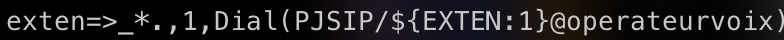
\includegraphics[width=0.7\textwidth]{img/exten-op.png}
		\caption{Configuration de l'opérateur voix dans extensions.conf}
		\label{fig:op-ext}
	\end{figure}\\
	\begin{itemize}
		\item \textbf{exten => \_.,1} signifie que cette extension est associée à tout numéro composé, quelle que soit la longueur et les chiffres qui le composent. Le "" signifie n'importe quel nombre et le "." signifie n'importe quelle longueur.
		\item \textbf{Dial(PJSIP/\${EXTEN:1}@operateurvoix)} signifie que l'appel sera acheminé via le protocole PJSIP en utilisant l'opérateur de voix défini. La variable "\${EXTEN:1}" est utilisée pour extraire le numéro composé par l'utilisateur, en excluant le premier caractère qui est un "\_".
	\end{itemize}

	\subsubsection{Validez les appels entrants et sortants entre cabinets médicaux}
	Suite à la configuration de l'opérateur voix, j'ai pu tester les appels entrants et sortants entre les différents
	cabinets de mes camarades. Tout est fonctionnel. Si par exemple je veux joindre
	Victor Uetwiller à la table7. Je compose \texttt{**72} et j'arrive bien
	à l'appeler. 

	\subsection{Appels externes}
	\subsubsection{Ajoutez les numéros à 10 chiffres pour les appels extérieurs via le faisceau}
	Pour pouvoir appeler à l'éxterieur de mon faisceau les appels à 10 chiffres, j'ai ajouté la ligne
	suivante dans le fichier \textbf{extensions.conf} :
	\begin{figure}[h]
		\centering
		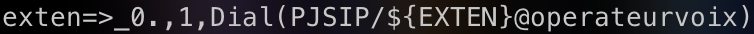
\includegraphics[width=0.7\textwidth]{img/externes.png}
		\caption{Configuration des appels à 10 chiffres extensions.conf}
		\label{fig:exter}
	\end{figure}\\

	\begin{itemize}
		\item \textbf{exten=>\_0.,1} définit le numéro de l'extension avec un masque de correspondance général, où \textbf{\_0.} signifie que cette extension sera activée pour tout numéro de téléphone commençant par \textbf{0}.\\
		\item \textbf{Dial(PJSIP/\${EXTEN}@operateurvoix)} est l'instruction pour composer un appel. \textbf{Dial} est une commande intégrée d'Asterisk qui permet de composer un appel vers une destination donnée. \textbf{PJSIP/\${EXTEN}@operateurvoix} est la destination de l'appel. \textbf{PJSIP} désigne le protocole de téléphonie IP utilisé (dans ce cas, PJSIP) et \textbf{\${EXTEN}} est une variable qui contient le numéro d'appel entrant (sans le "0" initial). \textbf{Operateurvoix} est le nom d'un serveur ou d'un fournisseur de services de téléphonie IP auquel l'appel doit être dirigé.
	\end{itemize}

	\subsubsection{Validez les appels externes vers (0112345678)}
	J'ai donc testé d'appeler les appels vers le 0212345678, le numéro hébergé par
	Victor sur son PC. Et l'appel fonctionne parfaitement. 

\end{document}